\chapter{Exigences fonctionnelles}

\section{Identification}

\begin{usecase}{Identification}

\begin{information}
\item[Acteur: ] Utilisateur
\item[Niveau:] Tâche principale
\item[Portée:] IHM, Base de donnée 
\item[Pré-condition:] L'utilisateur est non connecté et déja inscrit. 
\item[Post-condition:] L'utilisateur est connecté. 
\item[Priorité:] (5/5) : Cette étape est necessaire pour chacun des prochains cas d'utilisation.
\item[Fréquence:] Chaque lancement d'application.	
\end{information}	

\begin{scenario}
\item[1] L'utilisateur entre sont identifiant et son mot de passe,
\item[2] Il valide,
\item[3] L'utilisateur est connecté. 
\end{scenario}	

\begin{extension}
	\item[1]Renvoyer le mot de passe
	\item[2]Création d'un compte
\end{extension}
\end{usecase}

\begin{figure}[H]
  \begin{center}
  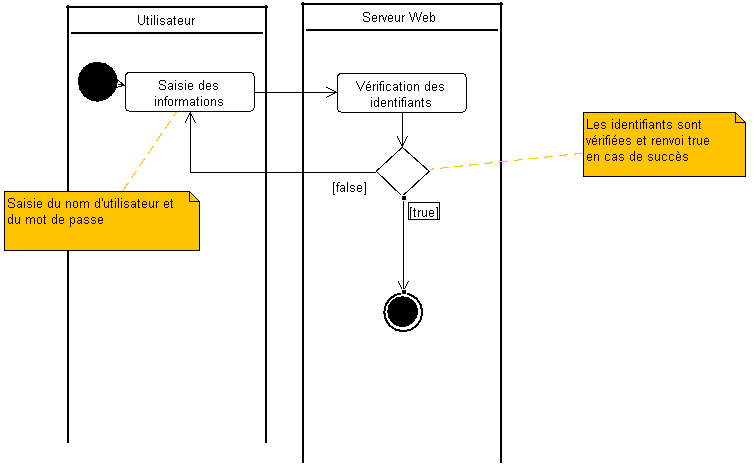
\includegraphics[scale=0.5]{diagrams/ActivityIdent.png}
  \caption{UML - Diagramme d'activitées - Identification}
  \label{fig:Architecture Generale}
  \end{center}
  \end{figure}

\subsection{Exigences fonctionnelles}
%<Itemize the detailed functional requirements associated with this feature. These are the software capabilities that must be present in order for the user to carry out the services provided by the feature, or to execute the use case. Include how the product should respond to anticipated error conditions or invalid inputs. Requirements should be concise, complete, unambiguous, verifiable, and necessary. Use “TBD” as a placeholder to indicate when necessary information is not yet available.>

%<Each requirement should be uniquely identified with a sequence number or a meaningful tag of some kind.>

%REQ-1:	
%REQ-2:
\begin{itemize}	\renewcommand{\labelitemi}{}
	\item \textbf{FONC11} - Saisie des identifiants,
	\item \textbf{FONC12} - Connexion (avec gestion de session),
	\item \textbf{FONC13} - Inscription,
	\item \textbf{FONC14} - Régéneration de mot de passe.\\
\end{itemize}

\section{Collect}

L'application n'a normalement pas à intervenir dans cette étape. Le recensement des idées est effectivement un processus utilisateur. Cependant, un pense-bête à idées non traitées par l'utilisateur peut s'avérer fort utile dans le cas où l'utilisateur est interrompu dans son processus.Un pense bête permet alors de stocker les idées non traitées.

\begin{usecase}{Collect}

\begin{information}
\item[Acteur:] Utilisateur
\item[Niveau:] Tâche principale
\item[Portée:] IHM, Base de donnée
\item[Partie prenante et interet :]
	Le recensement exhaustif de tout ce qui peut justifier une quelconque intervention de notre part : en suspens, inachèvement, en attente, intention, projet, manque, usure, mauvais fonctionnement, problème, in- satisfaction, besoin, engagements à tenir,etc.
Exemples : cette carte de visite restée dans une poche, cette facture dans la boîte à gants, cette demande reçue, ce dossier qui traîne sur le bureau, cette agrafeuse qui coince, cette course à faire, ce problème à résoudre, cette suggestion à tester, les messages de la boîte vocale, ce projet jamais réalisée, ce souci de santé, ce fauteuil qui grince, les performances de ce collaborateur, toutes ces choses en retard...
\item[Pré-condition:] Aucune. 
\item[Post-condition:] Les informations sont enregistrées dans l'application.
\item[Priorité:] (1/5) : Cette étape n'est pas indispensable, et peutêtre effectuer sans l'aide du système informatique.
\item[Fréquence:] Chaque début de journée.
\end{information}	

\begin{scenario}
\item[1] L'utilisateur après avoir effectuer sa reflexion, saisie les informations qu'il à recensée dans la boite à idée de l'application.
\end{scenario}

%\begin{extension}
%\item[1] 
%\end{extension}
	
\end{usecase}

% Utilisez le canevas de cockburn pour décrire le cas d'utilisation
% Indiquez la priotité: Haute, Moyenne et Basse
% Indiquez, éventuellement, des mesures spécifiques, comme le profit, le coût, les risques, etc. 
% (sur une échelle relative d'un minimum de 1 à un maximum de 9))

\subsection{Exigences fonctionnelles}

\begin{itemize}	\renewcommand{\labelitemi}{}
\item \textbf{FONC21} - Saisie des idées,
\item \textbf{FONC22} - Stockage des idées,
\item \textbf{FONC23} - Suppression des idées.
\end{itemize}


\section{Organisation des tâches}
	\begin{usecase}{Organize} 
		\begin{information}
			\item[Acteur :] Utilisateur
			\item[Niveau :] Tâche principale
			\item[Portée :] IHM, base de données
			\item[Pré-condition :] On dispose d''une liste de tâches issues du traitement des données.
			\item[Post-condition :] Les tâches appartiennent ou non à un projet, sont organisées en séquence ou non.
			\item[Priotité :] Haute
			\item[Fréquence :] Après chaque traitement des données.
		\end{information}
		\begin{scenario}
			\item[1] L'utilisateur regroupe les tâches par projet en fonction des propriétés communes de leurs contextes et de leurs intérêts communs.
			\item[1] Il peut aussi séquencer les tâches d'un projet. 
			\item[2] Il a aussi la possibilité de créer des sous-projets afin de donner un aspect hiérarchique au projet principal.
		\end{scenario}
		\begin{extension}
			\item[1]Si une tâche est isolée, elle n'appartient à aucun projet et n'est pas séquençable.
		\end{extension}
	\end{usecase}
		
	\subsection{Exigences fonctionnelles}
		Pour regrouper les tâches l'utilisateur doit pouvoir :
		\begin{itemize}	\renewcommand{\labelitemi}{}
			\item \textbf{FONC31} - créer/modifier/supprimer des projets,
			\item \textbf{FONC33} - affecter ou non des tâches à un projet,
			\item \textbf{FONC35} - affecter ou non des projets à un projet (sous-projets).
		\end{itemize}
		
	\subsection{Exigences non-fonctionnelles}
		\begin{itemize}	\renewcommand{\labelitemi}{}
			\item \textbf{FONC36} - Les tâches et sous-projets d'un même projet doivent participer à un même but.
			\item \textbf{FONC37} - Les tâches d'une même séquence doivent appartenir au même projet.
			\item \textbf{FONC38} - Les tâches et sous-projets d'un même projet doivent avoir des propriétés communes dans leurs contextes respectif.			
		\end{itemize}
		
		\begin{figure}[H]
			\begin{center}
				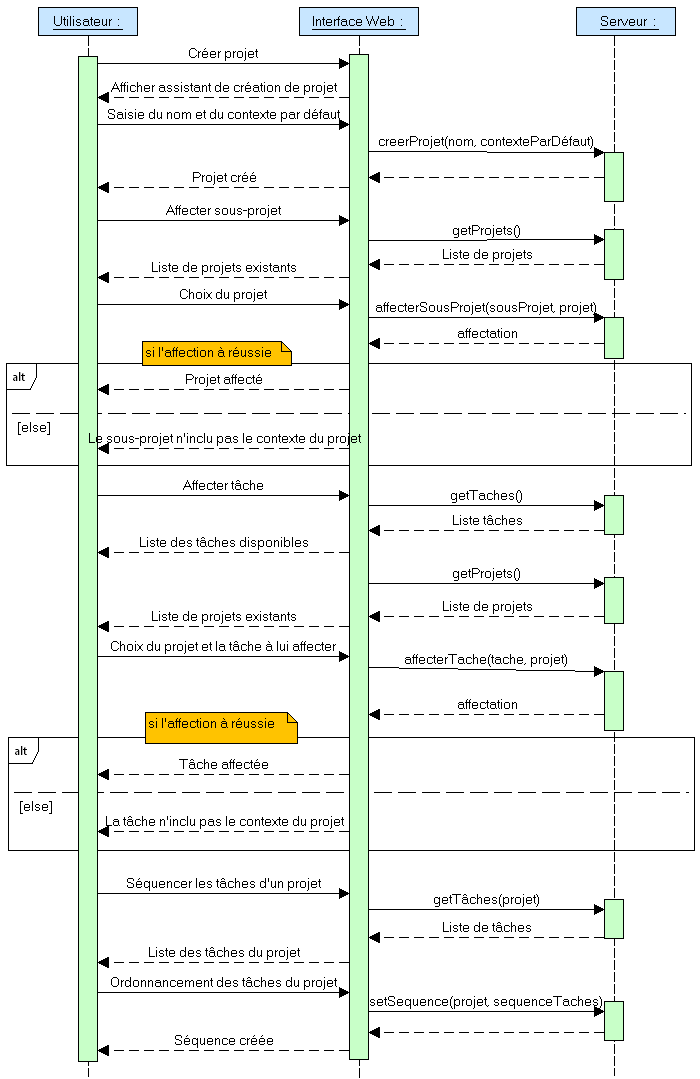
\includegraphics[scale=0.7]{diagrams/scenarOrganize.png}
				\caption{Diagramme de séquence de l'organisation des tâches}
			\end{center}
		\end{figure}		

\section{Affichage des tâches}
	\begin{usecase}{Affichage des tâches} 
		\begin{information}
			\item[Acteur :] Utilisateur
			\item[Niveau :] Tâche principale
			\item[Portée :] IHM
			\item[Pré-condition :] On dispose d'une liste de tâches, de contextes, de projets...
			\item[Post-condition :] Les tâches sont affichées selon les critères et vues choisies par l'utilisateur.
			\item[Priorité :] Haute
			\item[Fréquence :] Selon les besoins de l'utilisateur.
		\end{information}
		\begin{scenario}
			\item[1] L'utilisateur affiche les tâches qu'il effectuera selon les projets qu'il a choisit et le contexte courant.
			\item[2] Les tâches sont présentées de différentes manières (échéancier, agenda...).
		\end{scenario}
	\end{usecase}
	
	\subsection{Exigences fonctionnelles}
		L'utilisateur doit pouvoir via l'IHM :
		\begin{itemize}	\renewcommand{\labelitemi}{}
			\item \textbf{FONC71}- choisir les projets à réaliser.
			\item \textbf{FONC72}- sélectionner la ou les vues dans lesquelles seront affichées les tâches (échéancier, agenda...).
		\end{itemize}
		
\section{Réactualisation des tâches}
	\begin{usecase}{Réactualisation des tâches} 
		\begin{information}
			\item[Acteur :] Utilisateur
			\item[Niveau :] Tâche principale
			\item[Portée :] IHM, base de données
			\item[Pré-condition :] On dispose d''une liste de tâches.
			\item[Post-condition :] On délègue des tâches, celles finies sont supprimées, les vues sont mises à jour suivant le nouveau contexte, création automatique des tâches périodiques.
			\item[Priorité :] Haute
			\item[Fréquence :] Au moins une fois par jour.
		\end{information}
		\begin{scenario}
			\item[1] L'utilisateur change le contexte courant.
			\item[2] Indique les tâches effectuées.
			\item[3] Délègue des tâches.
		\end{scenario}
		\begin{extension}
			\item[2b] L'utilisateur peut annuler ses modifications.
		\end{extension}
	\end{usecase}
		
	
	\subsection{Exigences fonctionnelles}
		L'utilisateur doit pouvoir :
		\begin{itemize}	\renewcommand{\labelitemi}{}
			\item \textbf{FONC41} - mettre à jour le contexte.
			\item \textbf{FONC42} - indiquer les tâches réalisées.
			\item \textbf{FONC43} - délèguer une tâche.
			\item \textbf{FONC44} - revenir en arrière.
		\end{itemize}
		
		\begin{figure}[H]
			\begin{center}
				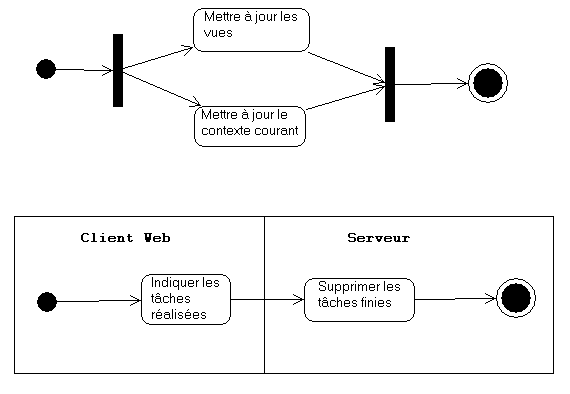
\includegraphics[scale=0.7]{diagrams/activiteReview.png}
				\caption{Diagramme d'activité de la réactualisation des tâches}
			\end{center}
		\end{figure}
		
		
%%%%%%%%%%%%%%%%%%%%%%%%%%%%%%%%%%%%%%%%%%%%%%%%%%%%%%%%%%%%%%%%%%%%%%%%%%%%%%%%%%%%%%%%%%%%%%%%%%%%%%%%%%%%%%%%%%%%%%%%%%%%%%%%%%%%%%%%%%%%%%%%%%%%%%%%%%%%
	
		
		
		
		
\section{Traitement des informations}
\begin{usecase}{Process}

\begin{information}
\item[Acteur: ] Utilisateur
\item[Niveau:] Tâche principale
\item[Portée:] IHM, Base de donnée 
\item[Pré-condition:] L'utilisateur est connecté au serveur web. 
\item[Post-condition:] Une tâche est créée sur les serveurs GTD et ToodleDo. 
\item[Priorité:] (5/5) : Cette étape est necessaire pour chacun des prochains cas d'utilisation.
\item[Fréquence:] De façon ponctuelle.	
\end{information}	

\begin{scenario}
\item[1] L'utilisateur regarde les éléments affichés dans sa boite à idées.
\item[2] L'utilisateur saisie les informations relatives à la tâche qu'il souhaite créer (nom, date debut, date fin, priorité, temps et energie requis ...).
\item[3] L'utilisateur crée la tâche.
\end{scenario}	

\begin{extension}
	\item[1]L'utilisateur oublie de remplir un champ obligatoire.
\end{extension}
\end{usecase}

\subsection{Exigences fonctionnelles}
%<Itemize the detailed functional requirements associated with this feature. These are the software capabilities that must be present in order for the user to carry out the services provided by the feature, or to execute the use case. Include how the product should respond to anticipated error conditions or invalid inputs. Requirements should be concise, complete, unambiguous, verifiable, and necessary. Use “TBD” as a placeholder to indicate when necessary information is not yet available.>

%<Each requirement should be uniquely identified with a sequence number or a meaningful tag of some kind.>

%REQ-1:	
%REQ-2:
\begin{itemize}	\renewcommand{\labelitemi}{}
	\item \textbf{FONC51} - Affichage de la boite à idées,
	\item \textbf{FONC52} - Saisie des informations relatives à une tâche,
	\item \textbf{FONC53} - Création d'une tâche,
\end{itemize}







\section{Synchronisation}
\begin{usecase}{Synchronisation}

\begin{information}
\item[Acteur: ] Serveur Web
\item[Niveau:] Tâche principale
\item[Portée:] Serveur GTD et ToodleDo et Serveur Web
\item[Pré-condition:] Le serveur web n'est pas synchronisé avec le serveur GTD ni ToodleDo
\item[Post-condition:] Le serveur web et les serveurs GTD et ToodleDo sont synchronisés
\item[Priorité:] (5/5) : Cette étape est necessaire pour assurer une persistance des informations.
\item[Fréquence:] A chacune des transactions
\end{information}	

\begin{scenario}
\item[1] L'utilisateur effectue une opération sur le client web
\item[2] Le serveur web enregistre les modifications utilisateur en mettant à jour sa base de données
\item[3] Le serveur web envoi les modifications effectuées aux serveurs
\end{scenario}	

\begin{extension}
	\item[1]La connexion entre les serveurs web et GTD et/ou ToodleDo est interrompue
	\item[2]La connexion entre les serveurs web et GTD et/ou ToodleDo se rétablie
\end{extension}
\end{usecase}

  \begin{figure}[H]
  \begin{center}
  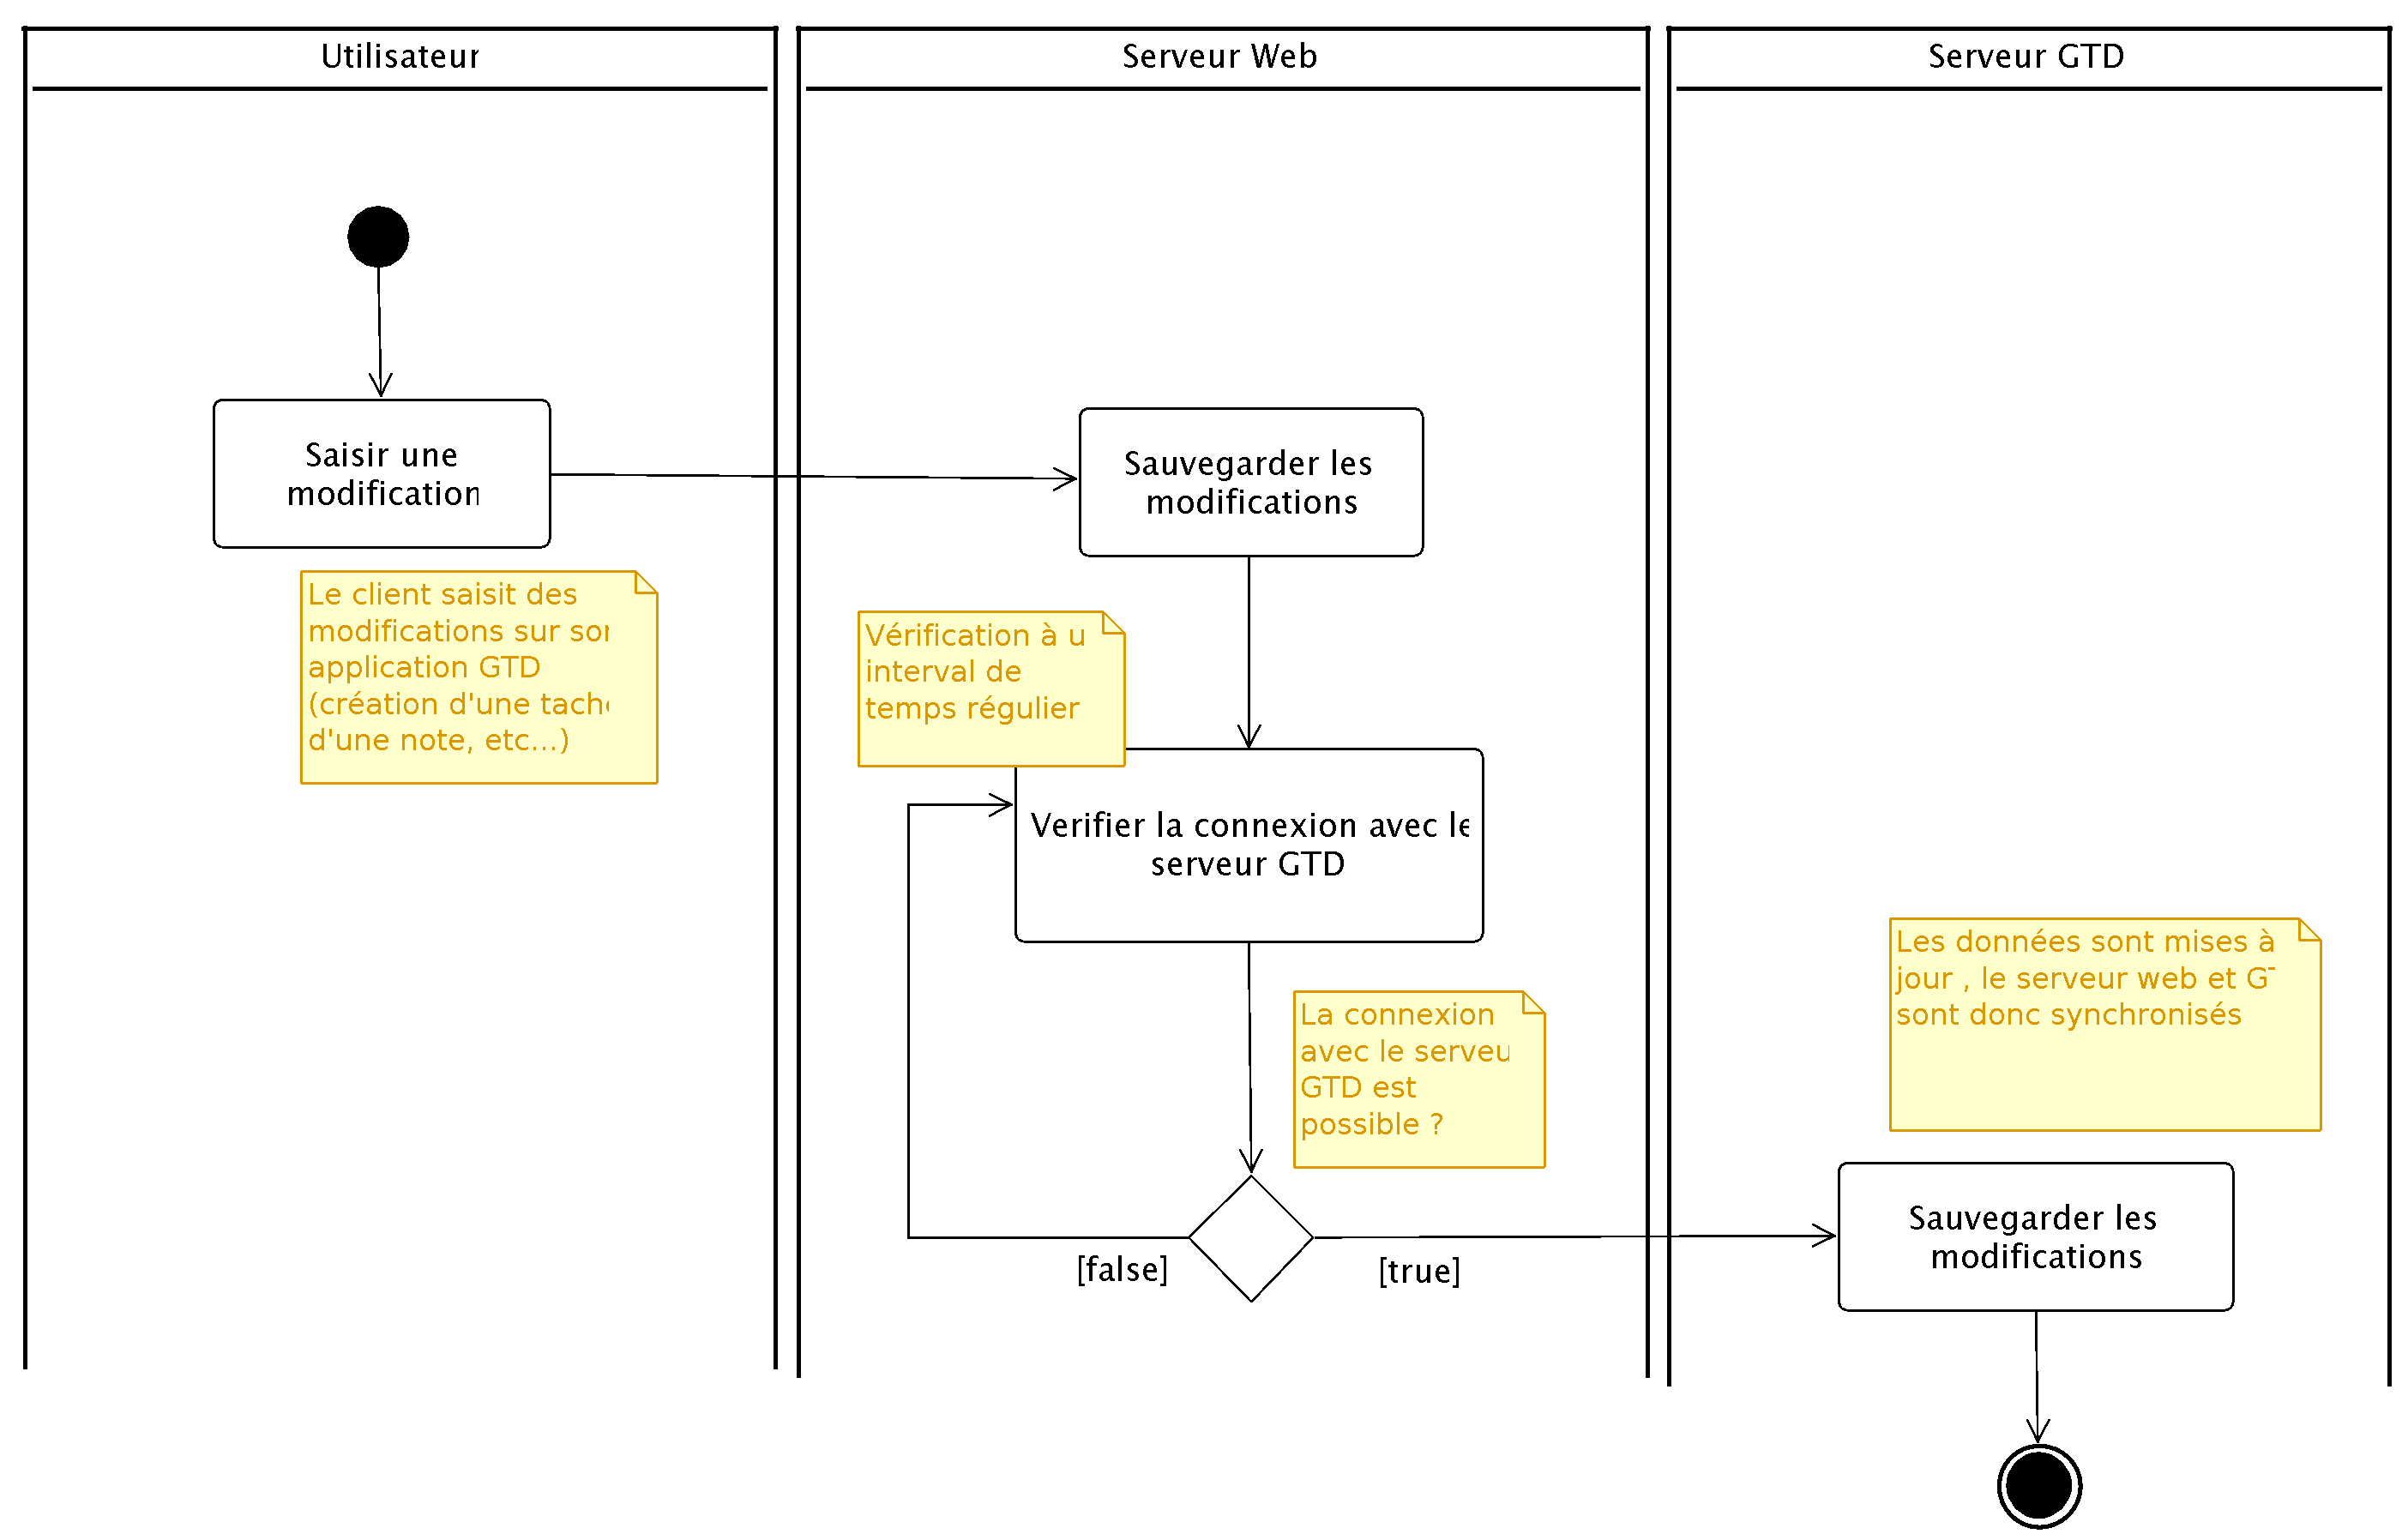
\includegraphics[scale=0.2]{diagrams/activiteSynch.png}
  \caption{UML - Diagramme d'activitées - Synchronisation}
  \label{fig:Architecture Generale}
  \end{center}
  \end{figure}

\subsection{Exigences fonctionnelles}
%<Itemize the detailed functional requirements associated with this feature. These are the software capabilities that must be present in order for the user to carry out the services provided by the feature, or to execute the use case. Include how the product should respond to anticipated error conditions or invalid inputs. Requirements should be concise, complete, unambiguous, verifiable, and necessary. Use “TBD” as a placeholder to indicate when necessary information is not yet available.>

%<Each requirement should be uniquely identified with a sequence number or a meaningful tag of some kind.>

%REQ-1:	
%REQ-2:
\begin{itemize}	\renewcommand{\labelitemi}{}
	\item \textbf{FONC61} - Enregistrement des modifications sur le serveur web,
	\item \textbf{FONC62} - Enregistrement des modifications sur les serveurs GTD et ToodleDo
	\item \textbf{FONC63} - Enregistrement des modifications sur les serveurs GTD et ToodleDo après une perte de connexion
\end{itemize}
		
